%----------------------------------------------------------------------------------------
%Capitolo 2 - Stato dell’arte: come risolvono gli altri questo problema? Quali sono le problematiche aperte?}
%----------------------------------------------------------------------------------------
This chapter is dedicated to the technical explanation of the two fundamental concepts for this thesis: Large Language Models (LLMs) and Prompt Engineering. As far as Large Language Models are concerned, we will start with an analysis of the development of Natural Language Processing (NLP), examining the evolution from the first systems to the current advanced models.
For Prompt Engineering, we will analyse the most commonly used categories, providing an overview of the techniques used in this study, which will be explored in greater depth in the following chapters.
In particular, Section \ref{sec:LLMs} will illustrate the concept of Large Language Models (LLMs), Section \ref{sec:Evolution} will examine Prompt Engineering in depth and, finally, the state of the art and practice of both technologies will be presented.

\section{Large Language Models}
\label{sec:LLMs}
\subsection{Language Model Evolution}
\label{sec:Evolution}

Language is one of the fundamental capacities of human beings, enabling communication and expression from the earliest years of life. In contrast, computers do not have an innate understanding of human language \cite{zhao2025surveylargelanguagemodels}.
However, Artificial Intelligence has made it possible to automatically process and generate language, allowing computers to interact with humans in an increasingly natural way \cite{Turing1950}.
This progress has been made possible thanks to the development of advanced tools, known today as Large Language Models (LLMs).
The evolution of Large Language Models (LLMs) did not happen overnight, but is the result of decades of research in the fields of Natural Language Processing (NLP) \cite{NLP} and Artificial Intelligence.
Before the introduction of the current models based on deep neural networks, several pioneering systems laid the foundations for the understanding and automatic generation of language, contributing significantly to the development of modern language technologies.
One of the first attempts to develop a programme capable of simulating a human conversation dates back to 1966, with the creation of ELIZA by Joseph Weizenbaum at MIT \cite{Segal_2025}.
ELIZA was a system based on pattern-matching \cite{PatternMatching} and predefined rules, designed to respond to users by adopting the communicative style of a Rogerian therapist.
Although its capacity for understanding was extremely limited, many users at the time interpreted its responses as a sign of supposed \textit{‘intelligence’}, highlighting the potential of conversational simulation techniques.
In the 70s, ELIZA's successor was PARRY, developed by Kenneth Colby \cite{parry2025}.
Unlike its predecessor, PARRY was designed to simulate the behaviour of a paranoid schizophrenic, integrating psychological models and more advanced rules. Thanks to these characteristics, the system was able to hold more believable conversations than ELIZA and was even subjected to experiments with psychiatrists. The results of these studies highlighted the ability of artificial intelligence to deceive human observers, demonstrating the potential of conversational simulations in the field of psychology and AI research.
At the same time, the linguist and computer scientist Terry Winograd developed SHRDLU \cite{winograd2025}, a system designed to understand and respond to commands in natural language within a simulated environment of virtual blocks.
This model demonstrated that, in a restricted and well-defined domain, a computer could process and manipulate language with a significant level of precision, highlighting the potential of the interaction between artificial intelligence and natural language.
In the 80s and 90s, advances in Machine Learning \footnote{\url{https://en.wikipedia.org/wiki/Machine_learning}} favoured the adoption of statistical models, including Markov chains and Hidden Markov Models (HMM) \cite{HMM},  in Natural Language Processing (NLP) \cite{NLP}.
These approaches formed the basis of advanced systems such as speech recognition and machine translation, and were applied in the first translation engines developed by IBM. However, these models had significant limitations, particularly in the management of extended linguistic contexts and in the understanding of semantics, hindering a deeper interpretation of human language.
The advent of deep neural networks marked a crucial turning point in natural language processing.
Techniques such as Word2Vec (2013) \cite{Word2vec} and GloVe (2014) \cite{Glove} allowed models to represent words in vector spaces, capturing semantic and contextual relationships. 
In this approach, words with similar meanings are close together in vector space, facilitating the construction of meaningful sentences.
Subsequently, the introduction of Long Short-Term Memory (LSTM) \cite{LSTM} and Recurrent Neural Networks (RNNs) \cite{Rnn} significantly improved the ability of models to handle longer text sequences.
RNNs \cite{Rnn} belong to a class of neural networks designed for processing sequential data, such as text or time series. Their main characteristic is the presence of recurrent connections, which allow them to maintain a ‘memory’ of previous information.
A Recurrent Neural Network (RNN) processes a sequence step by step, updating its hidden state \( h_{t-1} \)  according to the following update formula:\\
\begin{equation}
    h_t = \tanh(W_h h_{t-1} + W_x x_t + b)
\end{equation}
where \( W_h \) e \( W_x \) are the weights, \( x_t \) is the current input and \( h_{t-1} \) is the previous hidden state.
However, when the sequence becomes long, the problem of gradient disappearance \cite{Vanishing} arises, where the gradients can become too small or too large, making it difficult to train the models.
Long-short term memory (LSTM) \cite{LSTM}, as an evolution of RNNs \cite{Rnn},were designed to overcome the problem of short-term memory.
They use a special architecture with ‘gates’ that regulate the flow of information.
These gates are responsible for determining which information from the previous memory should be eliminated \textit{(Forget Gate)},  which should be added \textit{(Input Gate)}, which should be updated by combining Forget and Input \textit{(Cell State Update)} and, finally, which information should be sent as output \textit{(Output Gate)}.
Despite these improvements, LSTM models were still limited in their management of the global context of a text, hindering a deep understanding of the relationships between the various parts of a complex discourse.
\subsection{State-of-the-art}
\label{sec:stateoftheart}
In recent years, Large Language Models (LLMs) have revolutionised the field of artificial intelligence and Natural Language Processing (NLP) \cite{NLP}.
These language models, characterised by their considerable size, are neural networks trained on huge amounts of textual data and optimised to understand, generate and manipulate natural language in an increasingly sophisticated way.
Thanks to their ability to analyse complex contexts and produce coherent answers, LLM are used in a wide range of sectors, from automatic translation to virtual assistance and programming.
The evolution of these models has been made possible by advances in deep learning architectures, in particular with the introduction of Transformers \cite{Attention}  which have made it possible to overcome the limitations of traditional Recurrent Neural Networks (RNNs).
The architecture of a Transformer model is made up of two main components:\\
\begin{itemize}
    \item \textbf{Encoder}: The encoder consists of six identical layers, each of which includes two fundamental components: a multi-head self-attention mechanism and a fully connected feed-forward network applied position by position. It's task is to receive the input sequence of symbols, \( X = (x_1, x_2, \dots, x_n) \) and transform it into a continuous representation \( Z = (z_1, z_2, \dots, z_n) \).
    \item \textbf{Decoder}: The decoder is also made up of six identical layers. Unlike the encoder, each layer includes an additional multi-head attention mechanism that is applied to the output of the encoder, allowing the model to maintain memory of the input sequence. The decoder has the task of mapping the representation \( Z = (z_1, z_2, \dots, z_n) \) into the output sequence \( Y = (y_1, y_2, \dots, y_n) \) generating one element at a time.
\end{itemize}

\begin{figure}[h]
    \centering
    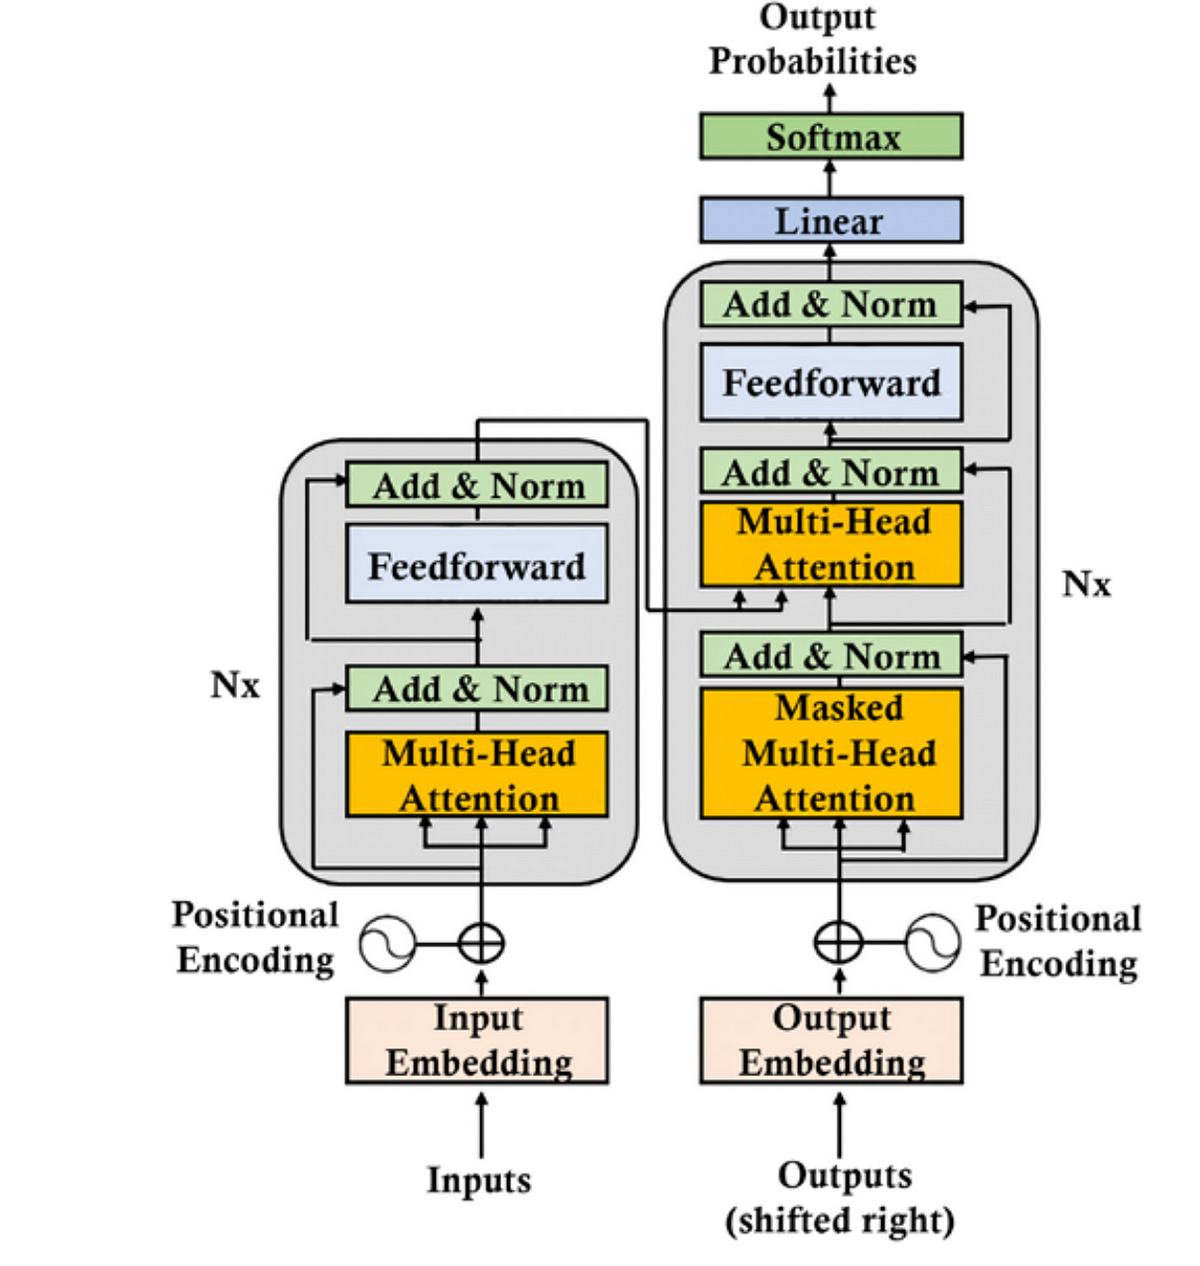
\includegraphics[width=0.7\linewidth]{Figures/Transformer.png}
    \caption{Transformer's architecture}
    \label{fig:graph}
\end{figure}
The original architecture of the Transformers is based on the combination of Encoder and Decoder. However, the architectures of the LLMs vary depending on the specific task that the model is intended to perform.
In particular, we can identify the following variants:\\
\begin{itemize}
    \item \textbf{Encoder-only}: These models are based exclusively on the architecture of the encoder, concentrating on text encoding for analysis and classification tasks. They form the basis for techniques such as text classification \cite{TextClassification} and Named Entity Recognition (NER) \cite{Ner}. Among the most popular models for such applications is \textbf{BERT} (Bidirectional Encoder Representations from Transformers) \cite{Bert}, which has gained wide recognition for its ability to understand the bidirectional context of text.
    \item \textbf{Decoder-only}:  Unlike the encoder-only models, these models only use the decoder part of a Transformer. They are mainly used in generating text from a sequence of inputs.  Among the best known examples are the \textbf{GPT} (Generative Pre-Trained Transformer) models, which stand out for their ability to generate coherent and fluid text in an autoregressive way.
    \item \textbf{Encoder-Decoder}: This category of models exploits both architectures of the Transformer, combining an encoder to analyse and understand the input and a decoder to generate the response output. They are used in tasks such as \textbf{Machine Translation} and \textbf{Text Summarisation}.
\end{itemize}
Before analysing the exposed LLM in detail, it is important to identify the key factors that influence their functioning and success: \\
\begin{itemize}
    \item \textbf{Tokenization}: The tokenisation process is a fundamental element in Natural Language Processing (NLP) models \cite{NLP}. Tokenisation consists of converting a structured text into small units, called tokens, which generally correspond to words or, in some cases, to single letters. This step is crucial for the algorithm, because through tokenisation and the subsequent creation of the embeddings, the model is able to understand more effectively the syntax of the sentence to be analysed.Today, modern LLMs use advanced algorithms such as \textbf{Byte Pair Encoding }(BPE) \footnote{\url{https://en.wikipedia.org/wiki/Byte_pair_encoding}} or WordPiece \cite{WordPiece} for tokenisation. \textbf{BPE} is a compression method that allows entire words or parts of words to be represented by a limited number of tokens, thus reducing the size of the vocabulary needed for model training.
    \textbf{Example}: \[
\texttt{'banana'} \rightarrow [\texttt{"b"}, \texttt{"a"}, \texttt{"n"}, \texttt{"a"}, \texttt{"n"}, \texttt{"a"}]
\]
Subsequently, in an iterative manner, the most frequent characters are counted and joined in a single representation:\\
\[
(\texttt{"b"}, \texttt{"a"}) \rightarrow 1 \text{ time}
\]
\[
(\texttt{"a"}, \texttt{"n"}) \rightarrow 2 \text{ times}
\]
\[
(\texttt{"n"}, \texttt{"a"}) \rightarrow 3 \text{ times}
\]
In this way the text is compressed and represented by more efficient tokens, combining characters and subwords.
\item \textbf{Embeddings}: Embeddings are continuous vector representations of words. The main objective of these representations is twofold. On the one hand, they are the only format that can be understood by artificial intelligence models, such as neural networks, to provide various types of input. On the other hand, representation in vector form allows the semantic relationships between words to be preserved, such as synonyms or analogies, allowing the model to understand and exploit these connections effectively during language processing.

\begin{figure}[h]
    \centering
    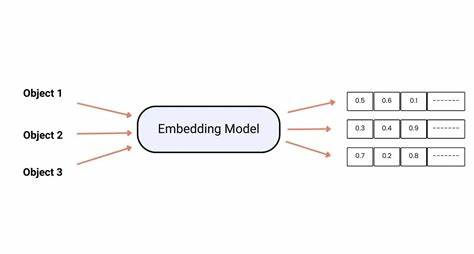
\includegraphics[width=0.7\linewidth]{Figures/Embeddings.png}
    \caption{Embedding's transformation}
    \label{fig:graph}
\end{figure}

\item \textbf{Attention}: As explained in the previous chapter, the attention mechanism used in Transformers allows the model to assign weights to words based on the context of the sentence. Thanks to this mechanism, the model is able to focus on the most relevant parts of the text, giving greater importance to crucial information, while ignoring the less significant parts.
\item \textbf{Pre-Training and Transfer Learning}: These two phases are crucial for the use of an LLM. Pre-training is a phase in which the model is trained on huge amounts of generic datasets, in order to teach it semantic relationships in various contexts: mathematical, logical, literal and so on. The strategy used for training models over the years has seen a considerable use of training data, called parameters. An increase in parameters leads to a greater understanding by the model, which, however, requires a longer training time. Transfer Learning is a methodology in which a model is first trained on a vast generic Dataset and then reused for more specific tasks with a limited amount of new data.This approach is particularly effective in Natural Language Processing (NLP)[19], where training models on huge amounts of text allows them to learn general linguistic representations, which can then be refined for specific applications. An example of Transfer Learning is \textbf{Retrieval Augmented Generation}(RAG)\cite{Rag} which uses knowledge of the pre-trained model to retrieve the most relevant information from new documents provided, specialising in an additional field of knowledge.

\end{itemize}

\begin{figure}[h]
    \centering
    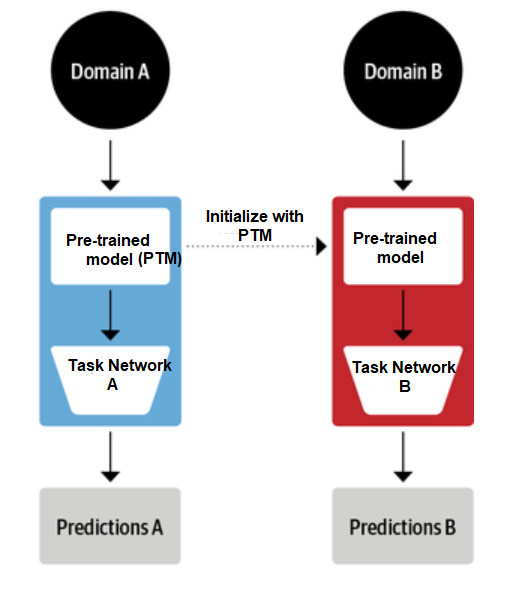
\includegraphics[width=0.7\linewidth]{Figures/Transferlearning.png}
    \caption{Transfer learning process between two domains \cite{vitalfluxNLP}}
    \label{fig:graph}
\end{figure}
Although the use of Large Language Models (LLMs) has brought significant advantages, such as quick access to a wide range of knowledge, these models are still subject to the phenomenon of hallucination. This phenomenon occurs when a model generates content that seems plausible but, in reality, does not correspond to the real facts.
An example of a hallucination is the following:\\
\\
\textbf{Question}: \textit{'Who invented the telephone'?}\\
\textbf{Answer}: \textit{'The telephone was invented by Thomas Edison in 1876.'}
\\
At first glance, the answer might seem correct. However, the statement is incorrect, as the telephone was invented by Alexander Graham Bell in 1876.
Hallucinations can be categorised into two main types\cite{Hallucination}:
\begin{itemize}
    \item \textbf{Intrinsic hallucinations}: these occur when the generated content directly contradicts the information provided in the input.
    \item \textbf{Extrinsic hallucinations}: these occur when the generated content cannot be verified with respect to the available sources. 
\end{itemize}
To mitigate the phenomenon of hallucinations, various strategies have been developed, including:\\
\begin{itemize}
    \item Improving the architecture of the model, to reduce systematic errors.
    \item Increasing the training parameters, to broaden the general knowledge of the model.
    \item Using advanced prompt engineering methods, such as Retrieval-Augmented Generation (RAG) \cite{Rag}, which integrates external sources to verify information.
\end{itemize}
\subsection{State of the practice}
Models such as GPT \footnote{\url{https://openai.com/index/chatgpt/}} and more recently LLaMA \footnote{\url{https://ai.meta.com/research/publications/the-llama-3-herd-of-models/}}, Mistral \footnote{\url{https://mistral.ai/en/news/mixtral-of-experts}} and Gemini \footnote{\url{https://gemini.google/?hl=en}} have marked fundamental stages in the development of this technology.
\textbf{GPT} is one of the most widely used and high-performing Large Language Models (LLM) currently available.
The GPT era began with GPT-1 \cite{GPT1} which, together with \textbf{BERT} \cite{Bert}  revolutionised the field of Natural Language Processing (NLP).
The success of these models inspired the creation of other architectures, such as \textbf{RoBERTa} \cite{Roberta} and \textbf{BART} \cite{BART}.
Both GPT-1 \cite{GPT1} and BERT \cite{Bert} have received widespread approval from the scientific community, demonstrating how human influence in the training process, traditionally based on manual labelling of data, was increasingly unnecessary thanks to the adoption of pre-training strategies on large quantities of unlabelled text. 
The evolution of these models led to the release of GPT-2 \cite{GPT2},which significantly improved NLP capabilities compared to its predecessor, being trained on a much larger number of parameters (about 1.5 billion compared to 117 million for GPT-1). This increase highlighted the crucial role of scalability in improving the performance of language models. 
The real leap in quality came with GPT-3 \cite{GPT3}, which introduced a model with 175 billion parameters, demonstrating unprecedented ability in natural language processing. However, the definitive turning point was the introduction of versions \textbf{GPT-3.5 (Turbo)}\footnote{\url{https://openai.com/index/gpt-3-5-turbo-fine-tuning-and-api-updates/}} and \textbf{GPT-4}\footnote{\url{https://openai.com/index/gpt-4/}}, made accessible through the online platform ChatGPT.
\begin{figure}[h]
    \centering
    
\includegraphics[width=0.7\linewidth]{Figures/Interfaccia.png}
    \caption{ChatGPT web interface}
    \label{fig:graph}
\end{figure}
These latest models not only excel in all the traditional NLP tasks, but also stand out for their ability to tackle logical-mathematical tasks and generate code, skills not initially foreseen by their developers\cite{kalyan2023surveygpt3familylarge}.
The evolution of GPT models shows how increased computational capacity and optimised architecture are key factors for the progress of artificial intelligence in the field of natural language processing. The models used in this work are GPT-3.5 (Turbo) and GPT-4o-mini, respectively a less expensive version than the GPT-4 version.
Furthermore, this latest version represents an improvement not only in terms of performance but also in terms of prompt generation. In fact, the latter belongs to the category of Multimodal models, which make the system capable of analysing and processing multiple types of data, such as text, images and sounds.
\begin{figure}[h]
    \centering
    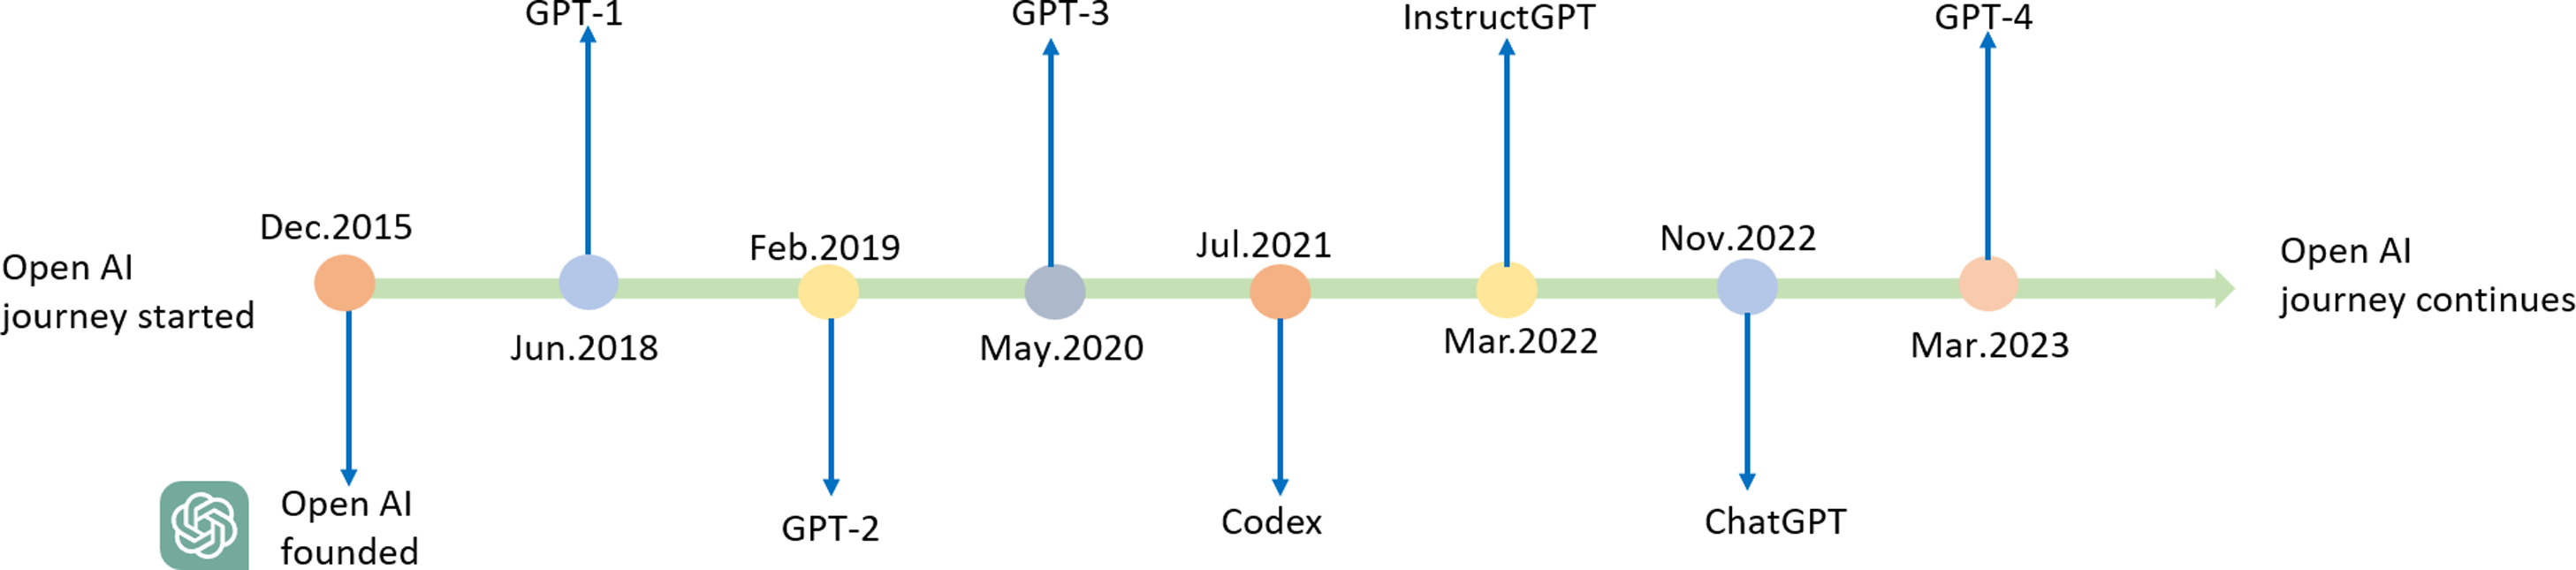
\includegraphics[width=0.7\linewidth]{Figures/Gpt.jpg}
    \caption{OpenAI's journey \cite{Journey}}
    \label{fig:graph}
\end{figure}

Gemini, also Google's proprietary software, was created as a Multimodal model, unlike GPT. This means that it is able to elaborate and process different types of input provided by users. The first version, Gemini 1.0, was released in 2023 in three variants with different architectures \cite{Gemini}: \\
\begin{itemize}
    \item \textbf{Gemini Ultra}: the most powerful model, designed to tackle complex tasks that require advanced reasoning.
    \item  \textbf{Gemini Pro}: a balanced version that offers a good compromise between performance and efficiency.
    \item \textbf{Gemini Nano}: designed for mobile devices, it allows you to perform artificial intelligence operations directly on the devices.
\end{itemize}
A few months later, Google introduced the Gemini 1.5, 1.5 Pro and 1.5 Flash versions, characterised by significant improvements in reasoning capabilities and greater processing speed. These models are based on a different architecture from the previous ones, called \textbf{Mixture of Experts}(MoE)\cite{MoE}.
\begin{figure}[h]
    \centering
    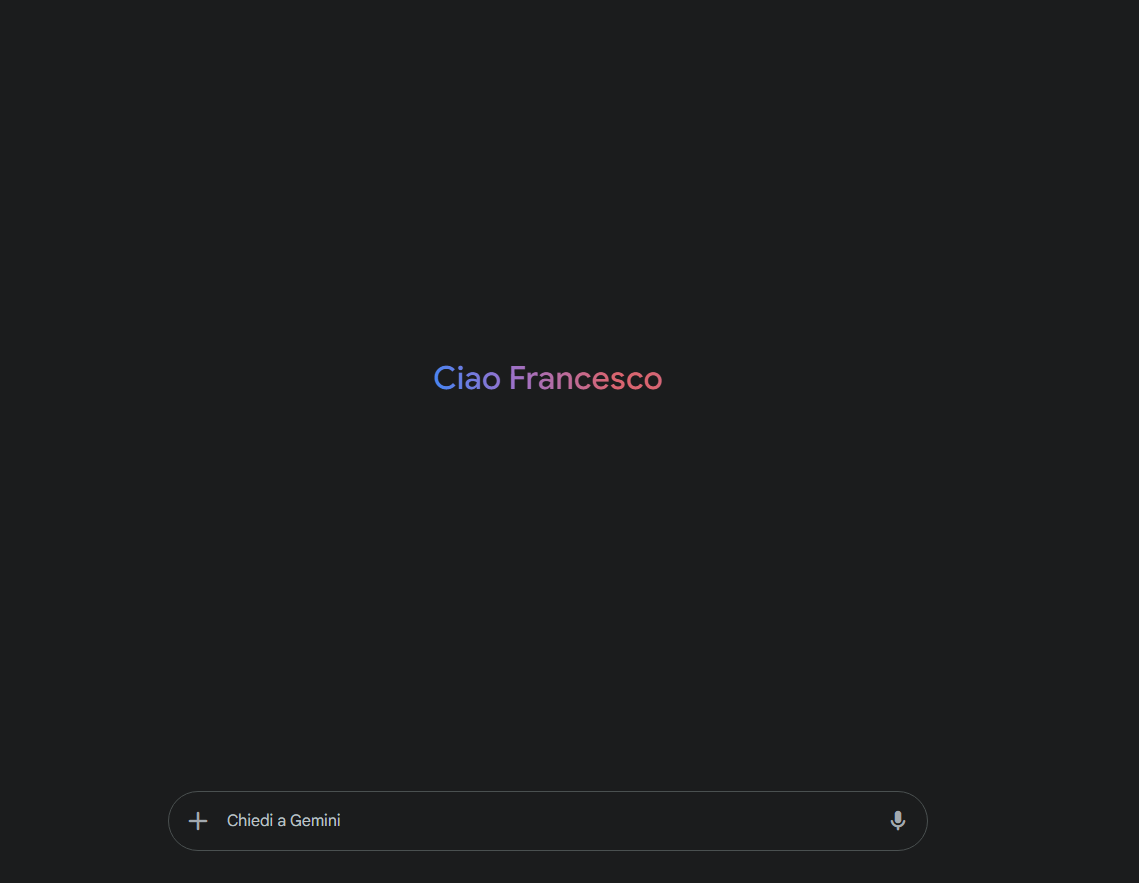
\includegraphics[width=0.7\linewidth]{Figures/Gemini.png}
    \caption{Gemini web interface}
    \label{fig:graph}
\end{figure}
The MoE architecture differs from traditional Transformers in that it has a modular approach: the neural network is divided into different ‘experts’, each specialised in a specific task. Based on the user's request, Gemini dynamically selects the most suitable experts, thus improving the quality and efficiency of the generated responses.
Starting in 2023, Meta AI \footnote{\url{https://ai.meta.com/}}, in order to keep up with the competition in the development of Large Language Models (LLMs), suitable for the development of an \textbf{Artificial General Intelligence} (AGI)\cite{AGI}  released the \textbf{Large Language Model MetaAI} model, later stylised as \textbf{LLaMA}.
Initially, this model was released to the research community with a non-commercial licence. Subsequently, following unauthorised shared copies, it was made completely open-source. The power of this LLM lies in the fact that it is small and fast, compared to other LLMs in the sector. In fact, any user with a high-performance GPU can test it on their computer.
The first versions of LLaMA, 7B and 65B, showed exceptional results compared to the GPT-3 versions, despite being over ten times smaller \cite{touvron2023llamaopenefficientfoundation}.
The subsequent versions, LLaMA 2 and LLaMA 3 and 3.1, differ both from the GPT (with Transformer) and Gemini (with MoE) approaches. The architectural development of Llama is based on two main parts:\\
\begin{itemize}
    \item \textbf{Pre-training}: initial training phase in which, as with the other models, the LLM is trained on a massive amount of data to ensure that it learns the semantic connections as well as possible.
    \item \textbf{Post-training}: next phase in which human feedback is inserted with a Reinforcement Learning (RL) approach [49] using a technique called \textbf{Direct Preference Optimisation}(DPO) \cite{rafailov2024directpreferenceoptimizationlanguage}.
    With this method, after pre-training, the original model is trained to recognise the best responses, chosen using a human approach. Compared to classic \textbf{Reinforcement Learning} (RL) where another model is created from human responses, here the best responses are selected directly, making the approach faster.   
\end{itemize}
The Mistral AI models, like LlaMa's, are also open-source. Mistral has quickly established itself as one of the main players in the field of LLMs, competing with OpenAI, MetaAI and Google. 
Its philosophy is based on light, efficient and open-source models with a focus on high performance and accessibility. The first model released was \textbf{Mixtral 7B} \cite{Mixtral7b} with 7 billion parameters.
Although smaller than its competitors at the time (LLaMA 2 and Gpt-3.5), it offered competitive performance.
Later, the \textbf{Mixtral 8x7B}\cite{Mixtral8} was released, which was used in this thesis.
This model,based on the Mixture of Experts architecture, is composed of 8 experts, of which 2 are activated for each token, resulting in an effective capacity of 12-14 billion parameters during inference.
\begin{figure}[h]
    \centering
    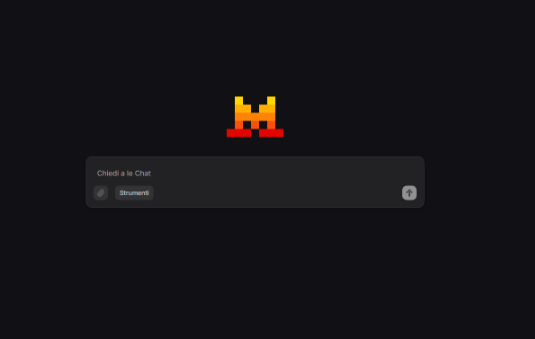
\includegraphics[width=0.7\linewidth]{Figures/Mixtral.png}
    \caption{Mixtral web interface}
    \label{fig:graph}
\end{figure}
The last model analysed is \textbf{DeepSeek}, which, unlike the other models mentioned above, was used in this thesis as a judge for the evaluation of the results, the methodology of which will be explained in detail in the following chapters.
DeepSeek is a Chinese company specialising in the development of Artificial Intelligence models. Initially founded in 2016, it didn't take on its current name until 2023. Despite its recent success in the sector, the company quickly managed to adapt to the competition, releasing its first model, \textbf{DeepSeek-Coder}, in 2023, followed by the development of versions \textbf{V2} and \textbf{V3} at the end of 2024.
The DeepSeek V3 model, like Mixtral 8x7B and Gemini 2.0, adopts a Mixture of Experts (MoE) architecture, characterised by 671 billion parameters, of which 37 billion are activated for each token processed by the various experts. This model has distinguished itself as one of the highest performing state-of-the-art models, demonstrating superior reasoning ability in various benchmarks compared to other advanced models such as \textbf{Claude 3.5}\footnote{\url{https://www.anthropic.com/news/claude-3-5-sonnet}} and \textbf{GPT-4o}.
Despite its high performance, the training process of DeepSeek required only a tenth of the hours used for training GPT-4o \cite{Deepseek}.
This result was also possible thanks to the use of 8-bit FP8 precision, which provides a more compact numerical representation compared to the standard FP16 or FP32. This approach allows for a significant reduction in memory usage and an increase in calculation speed, making DeepSeek V3 extremely efficient in terms of both performance and computational resources.
\begin{figure}[h]
    \centering
    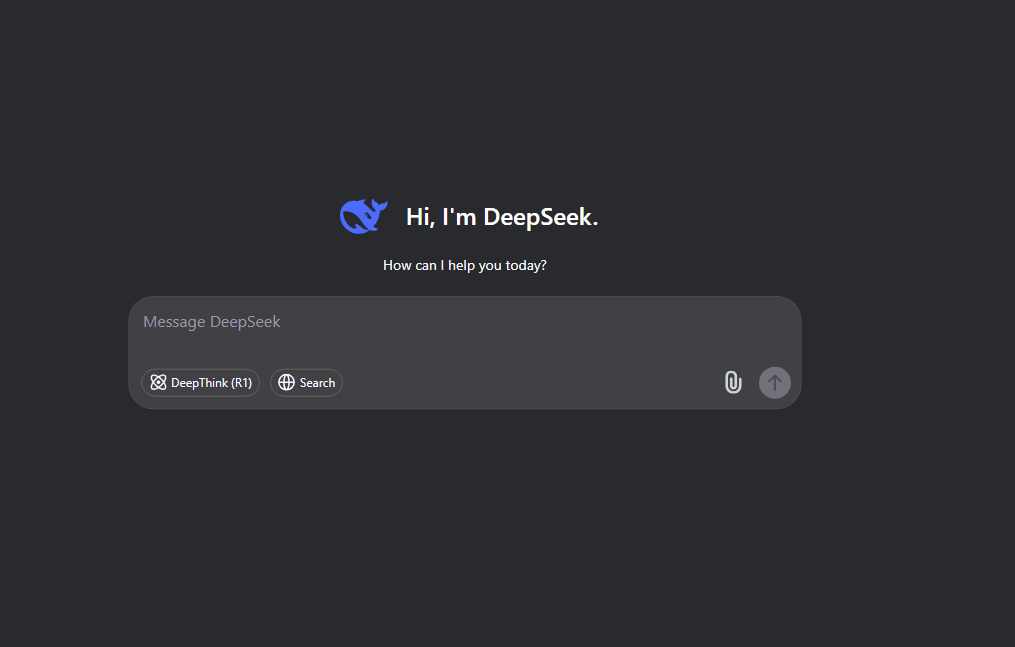
\includegraphics[width=0.7\linewidth]{Figures/DeepSeek.png}
    \caption{DeepSeek web interface}
    \label{fig:graph}
\end{figure}

\section{Prompt Engineering}
\label{sec:Prompt}
In this section we will explain what Prompt Engineering is, starting with an analysis of its origin and its evolution over time. We will then provide an overview of the main techniques, highlighting their differences and their impact on results in the different areas of application of Large Language Models.
\subsection{Introduction and Evolution}
Prompt engineering is now a fundamental discipline in the interaction with Large Language Models (LLMs), as it allows us to optimise responses, control the behaviour of Artificial Intelligence systems and adapt them to specific contexts. Its roots lie in Claude Shannon's Information Theory (1948) \cite{IT}, which laid the foundations for the efficient encoding and transmission of information, laying the basis for the subsequent evolution of Information Retrieval systems.
Already in the 50s and 60s, with the development of the first statistical models of language, such as \textbf{n-grams}\footnote{\url{https://it.wikipedia.org/wiki/N-gramma}}, began to explore the possibility of predicting subsequent words based on probability, while in the 70s and 80s text search systems used structured queries to retrieve information from large databases.
These systems, although rudimentary by today's standards, can be considered an early form of prompting system, as they required the user to formulate precise requests in order to obtain relevant results.
The advent of neural networks and machine learning marked a major turning point in Natural Language Processing (NLP) \cite{NLP}, enabling the transition from traditional statistical models to vector representations of words. With the introduction of word embeddings (Word2Vec, 2013) \cite{Word2vec}, Natural Language Processing (NLP) acquired a greater capacity for contextual understanding, paving the way for systems capable of generating text in a more natural and coherent way.
However, the real revolution occurred with the introduction of the Attention Mechanism \cite{Attention}, and the Transformer models, which allowed the models to process information with a global view of the context, drastically improving the quality of text generation.
Today, with the spread of Large Language Models (LLMs) such as GPT-4, Prompt Engineering represents a set of techniques aimed at perfecting the formulation of the request to obtain more accurate results. This has become an essential element in guiding models towards more coherent, controlled and personalised outputs. This has enabled more effective interaction between humans and machines, allowing the use of models in critical areas such as medicine, law and scientific research. At the same time, growing awareness of the social implications of AI has led to an increasing focus on the need for responsible prompt engineering, capable of mitigating bias, improving transparency and ensuring the safe use of language models \cite{schulhoff2025promptreportsystematicsurvey}.
Modern prompting techniques are not limited to providing simple textual input, but include advanced strategies to induce the model to respond in a more structured and precise manner.
\subsection{Taxonomies and main techniques}
Although this is a relatively new and constantly evolving field, the role of the prompt engineer, is becoming increasingly important, thanks to his ability to optimise interaction with linguistic models. A competent prompt engineer must be able to analyse the context in which the model is used and, consequently, apply the most appropriate prompting technique to maximise the effectiveness and accuracy of the responses.
Currently, prompt engineering techniques can be organised within a well-defined taxonomy, which classifies the main strategies:\\
\begin{itemize}
    \item \textbf{Zero-shot}: includes all techniques in which the prompt is formulated without including examples of any kind, relying exclusively on prior knowledge of the model.
    \item \textbf{Few-shot}: is based on inserting examples within the prompt to provide the model with a clearer context and improve its ability to understand and generalise.
    \item \textbf{Thought Generation}: includes strategies aimed at stimulating the model to generate a structured reasoning process, improving the consistency and quality of the responses.
    \item  \textbf{Ensembling}:involves exploring different approaches to solving the problem, then combining the answers obtained and selecting the most appropriate one.
    \item \textbf{Retrieval Augmented Generation}: involves the creation of retrievers \cite{Rag} from which the models can draw in order to correctly answer questions.

\end{itemize}
This classification allows us to outline more clearly the different methods used in Prompt Engineering, facilitating their application in specific contexts.
The \textit{zero-shot} methodology is characterised by the formulation of a question without including examples of answers, relying entirely on the previous knowledge of the model to generate a relevant output.\\
\\
\textbf{Example}:\\
\textbf{Question}: \textit{'Classify this sentence as neutral, positive or negative.'}\\
\textbf{Text}: \textit{'I think it was a nice holiday'}\\
\textbf{Sentiment}:\\
\\
In this context, the Large Language Model (LLM) that is given the following prompt will simply have to identify the sentiment of the question, based solely on the combination of tokens that make up the sentence. Several more advanced approaches have been developed based on this methodology.
One example is \textbf{Emotion Prompting}\cite{Emotionprompt}, a technique that integrates emotional elements into the prompt in order to influence the model's response. The idea behind this strategy is that models can generate more accurate and engaging results if the prompt includes emotional references. This is because, through the use of words associated with specific emotions, the model can draw on similar texts present in the training data, improving the relevance and quality of the responses.\\
\\
\textbf{Example}: \\
\textbf{Normal Question}: \textit{'A friend says: ‘I feel very sad today. Reply'}\\
\textbf{Emotion Prompting}: \textit{'A friend says: ‘I feel very sad today’. Offer words of comfort, showing that you are considerate and willing to help.'}\\
\\
Another methodology developed from \textit{zero-shot} is \textbf{Role Prompting} \cite{Role}, a technique adopted in this thesis and which will be explored in more detail in the Chapter \ref{cap:progettazione}.
Several studies have shown that increasing the number of examples provided within the prompt can significantly improve the overall performance of the models \cite{schulhoff2025promptreportsystematicsurvey}.
In particular, the greater the number of examples included, the greater the benefit for the model. This strategy falls under the category of \textit{few-shot prompting}, which exploits the ability of LLMs to learn new patterns without the need for further fine-tuning, relying exclusively on the examples provided.
The simplest case of this methodology is \textit{one-shot prompting}, in which the prompt includes a single example of a response, allowing the model to adapt to the required task with minimal contextual input.\\
\\
\textbf{Example}: \\
\textbf{Question}: \textit{'Classify this sentence as neutral, positive or negative.'} \\
\textbf{Example 1}: \textit{'I hate when all day rain.'} -> \textbf{Sentiment}: \textit{Negative}\\
\textbf{Text}: \textit{'The sun is shining and I feel happy.'} -> \textbf{Sentiment}: \\
\\
Few-shot prompting follows the same structure as one-shot prompting, but includes a greater number of examples. Over the years, further advanced approaches have been developed from this methodology, including \textbf{Self-Generated In-Context Learning}(SG-ICL)\cite{kim2022selfgeneratedincontextlearningleveraging}.
This technique is particularly useful when there are no predefined examples to provide to the model. Instead of drawing on an external dataset, the model autonomously generates relevant examples before responding to the main request. The idea behind this strategy is that the self-generation of relevant examples for a specific use case can significantly improve the quality of the final response.
Another advanced technique belonging to the few-shot prompting category is \textbf{K-Nearest Neighbour Prompting}(KNN) \cite{xu2023knnpromptingbeyondcontextlearning}, in which the examples provided to the model are selected dynamically based on their similarity to the input. The process generally consists of the following phases:\\
\begin{enumerate}
    \item Creation of a dataset of examples.
    \item Vector representation of the examples.
    \item Calculation of similarity, using metrics such as \textit{cosine similarity}, or \textit{Euclidean distance}.
    \item Selection of the k closest examples.
    \item Construction of the final prompt.
\end{enumerate}
This approach allows for improving the adaptability of the model to specific requests, guaranteeing more coherent and pertinent answers.
Among the techniques belonging to the \textbf{Thought Generation} category, one of the most important is the \textbf{Chain-of-Thought} (CoT)\cite{Cot}.
This methodology is designed to guide the model in the development of a more structured reasoning process, with the aim of improving the accuracy and reliability of the generated responses. This technique simulates the way humans think sequentially. When a person solves a problem, they usually follow these steps:\\
\begin{enumerate}
    \item Breakdown of the problem into simpler parts.
    \item Logical reasoning for each steps.
    \item Linking information to reach a conclusion.
\end{enumerate}
For example, a child learning to add \textit{12+15} might say: \textit{'I know that 10 + 10 makes 20’, ‘then I add 2 and get 22’, ‘finally I add 3 and arrive at 25'}.
This natural form of reasoning is reproduced in CoT \cite{Cot}. 
This technique is particularly useful in more complex analyses, in which the models tend to have more gaps, both due to a limited availability of data and because of their probabilistic nature, which leads them to generate the most plausible answer without necessarily following a logical reasoning process.This is particularly evident in areas such as the resolution of mathematical and logical problems, medical diagnoses and, more generally, in legal contexts, as in the case of the present thesis work.
There are several variations of the Chain-of-Thought (CoT) approach, including \textit{zero-shot CoT},in which no explicit examples are provided, but the model is invited to develop structured reasoning through explicit instruction, such as \textit{let's think step by step}. 
For example, let's consider the following case:\\
\\
\textbf{Question}: \textit{'If a bus leaves at 14:30 and takes 2 hours and 45 minutes to reach its destination, what time does it arrive? Let's think about it step by step.'}\\
\\
This approach is particularly useful for relatively simple problems, such as the example given. However, its effectiveness tends to decrease in more complex scenarios, where the model may require concrete examples to refine the reasoning process and improve the accuracy of the response.
To support this limitation, \textit{few-shot CoT},  is used, a variant in which examples are provided within the prompt to guide the model to develop a reasoning process similar to that illustrated in the proposed examples. This approach has proven particularly effective in refining the inferential capabilities of the models, improving the accuracy of responses in more complex contexts.
A further extension of the \textit{Chain-of-Thought} is the \textit{Tree-of-Thought} \cite{ToT},a methodology in which the model does not follow a single line of reasoning, but explores several alternative paths before selecting the most appropriate response.
This approach allows us to evaluate different resolution strategies, increasing the robustness and reliability of the generated responses. Another interesting approach in the Thought Generation category is the \textbf{Step-Back prompt} \cite{Stepback}.
This technique encourages the model to take a step back and reflect on more general concepts before solving a specific problem. Here too, as with the other techniques, the aim is to improve reasoning, but by making it analyse a problem from a broader perspective.
Here's an example to help you understand better:\\
\\
\textbf{Question}: \textit{'If a circle has a radius of 5 cm, what is its area? Before answering, explain the concept of the area of a circle'}.\\
\\
In this way, the answer could be correct both normally and with this approach, but by doing this the model demonstrates a deeper and more structured understanding.
As for the category \textbf{Ensembling}, as mentioned above, it refers to a technique that combines different prompting approaches to obtain more accurate responses from the models. 
The idea is therefore to assemble or combine several prompts, to exploit the strengths of each one. Among these techniques we find \textbf{self-consistency} \cite{SC}, also used in this thesis work, which is one of the most used techniques and generates more reasoning paths, which will be explained in Chapter \ref{cap:progettazione}.
Another technique, an extension of the Mixture of Experts (MoE) \cite{MoE} architecture, on which some modern models are based, is the \textit{Mixture of Reasoning Experts} (MoRE) \cite{MoRE}.
The central concept behind this methodology is to combine different \textit{experts} specialised in specific areas of reasoning to improve the quality of the answers generated by the model.
Each \textit{expert} provides an answer to the question based on their area of expertise.
For example, for the question \textit{'How do I produce my own homemade gin?'},  the model could ask for the intervention of the expert in legal regulations, the expert in chemical processes and distillation, and the expert in botany. The model will then select the answer of the expert deemed most reliable based on the context of the question.
Finally, the last prompting technique analysed is \textbf{Retrieval Augmented Generation }(RAG)\cite{Rag}.
Large Language Models can be used to carry out different types of daily activities, such as classification, sentiment analysis and, in the case of \textbf{Multi-Modal Large Language Models} (MLLMs)\cite{Yin_2024}, also image, video and audio generation. However, their knowledge in some specific sectors may be limited, such as in the medical sector.To overcome this problem, RAGs are used. A RAG is a system that combines a retrieval component called a retriever with the use of Large Language Models. These models use, as input, documents relevant to a given case study, which are concatenated to the prompt to generate a more informative final response. This methodology allows Large Language Models to avoid fine-tuning on a given specific context and therefore use the most up-to-date knowledge contained within the documents to answer the original question.

\begin{figure}[h]
    \centering
    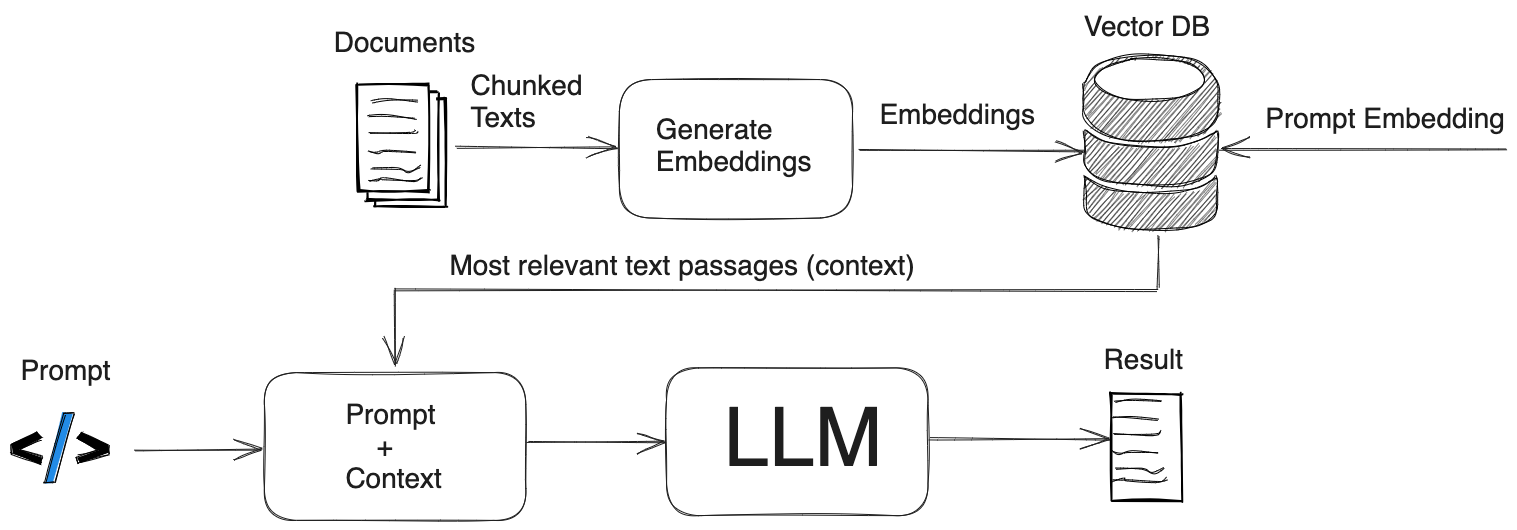
\includegraphics[width=0.7\linewidth]{Figures/RAG.png}
    \caption{RAG's elaboration process.}
    \label{fig:graph}
\end{figure}
The way this technique works is best illustrated in Figure 2.9:\\
\begin{enumerate}
    \item \textbf{Retrieval of documents}: in this phase, the user is asked to retrieve the documents most relevant to the case study in question. For example, in the context of the question \textit{'How do I make my own homemade gin?'},the user could retrieve informative documents relating to the creation of spirits and the regulations in force in his/her geographical area.
    \item \textbf{Creation of the Vector DB}: next, the collected documents are transformed into vector embeddings as described in Section \ref{sec:stateoftheart}. These embeddings are then used to create a Vector Database (Vector DB) that contains the external knowledge derived from the documents.
    \item \textbf{Generation}: In the last phase, the prompt is enriched with the context extracted from the Vector DB, which is used to improve the model's ability to generate a more precise and contextualised response.  
\end{enumerate}

However, although this technique is particularly advantageous in contexts where Large Language Models are not updated, it has some critical aspects. These include the complexity of implementation and maintenance, as a continuous process of document retrieval and reconstruction of the Vector DB is necessary to ensure that the system is always up to date. In addition, computational costs and latency times must also be considered: if the Vector DB is particularly large or the connection to it is slow, the response time of the model can increase, negatively compromising the user experience.

\subsection{State-of-the-practice}
\label{sec:stateofthepractice}
The use of Prompt Engineering has found concrete applications in various sectors, significantly improving the effectiveness of Large Language Models. Some of the fields in which these techniques are used successfully include medicine, education and law.

\subsubsection{Prompt engineering in the medical field:}
The use of prompt engineering techniques is enjoying growing success in various areas, including medicine. The latter is a highly specialised domain and poses significant challenges in the generation of accurate outputs by Large Language Models (LLM). Several studies have applied prompt engineering to various medical tasks, including the classification of clinical texts, the generation of new medical content (texts, images and clinical reports) and Question Answering,  i.e. the ability of models to answer medical questions \cite{wang2021prompt}.
In the \textit{HealthPrompt}\cite{sivarajkumar2022healthpromptzeroshotlearningparadigm} study, the authors adopted an approach based on Zero-Shot Learning (ZSL) as a prompt engineering strategy to classify clinical texts using six different LLM. The results show that, even without fine-tuning on specific data, the models were able to recognise the medical context and classify the clinical documents based on the phenotype to which they belonged, such as obesity, heart disease, depression and alcohol abuse.
In another study \cite{lamichhane2023evaluationchatgptnlpbasedmental}, GPT-3.5 Turbo was used in combination with a prompt in zero-shot mode to classify texts from social media into three distinct categories aimed at recognising mental health conditions: depression detection, stress detection and suicidality detection.
In the \textit{ChatAug}\cite{dai2023auggptleveragingchatgpttext} projects, several prompts were developed and used with the aim of auto-generating new data, which was then used in few-shot prompting techniques. The automatic generation of data is particularly important in the medical field, where there is often a limited availability of annotated datasets.
In \textit{Med-PaLM} \cite{tuli2023large} using the \textit{PaLM} model \cite{Palm}  and prompt engineering techniques, the authors designed a system to answer multiple-choice questions on several reference datasets, including \textit{MedQA}, \textit{MedMCQA} and  \textit{PubMedQA}. The system's performance was compared with the answers provided by doctors, showing promising results.
\subsubsection{Prompt engineering in the educational field:}
In education, the use of Large Language Models (LLM) and Prompt Engineering techniques offers revolutionary opportunities for learning and teaching. These tools can support students and teachers in understanding complex concepts, creating teaching materials and automating repetitive tasks, such as correcting homework. The adoption of these technologies not only facilitates access to educational resources on a large scale, but also promotes a more interactive and inclusive learning experience, adaptable to the needs of each teacher and student.
For example, in \cite{lee2025prompt} the role of Prompt Engineering and Artificial Intelligence in secondary education is analysed, highlighting how these techniques can improve both teaching and learning.
Another study \cite{woo2024effectspromptengineeringintervention}investigated the effectiveness of university students using LLM to understand concepts related to Artificial Intelligence, showing a significant increase in their ability to assimilate these notions.
In \cite{baldassarre2024didattica} the impact of Prompt Engineering on university students was examined, with the aim of assessing how its use influences self-efficacy, i.e. the ability to master and successfully perform a specific task in the field of Artificial Intelligence. The results showed an improvement in self-efficacy, a greater understanding of the key concepts and better ability to formulate effective prompts.
These studies demonstrate the importance of Prompt Engineering in training, optimising the use of Artificial Intelligence systems, in particular Large Language Models, which today represent a central resource in society.

\subsubsection{Prompt Engineering in the legal field:}
In the legal sector, the use of Large Language Models (LLMs) combined with Prompt Engineering techniques is widespread to support lawyers in drafting legal documents and in decision-making processes. However, the current use of these models is mainly focused on facilitating the creation of legal texts or assisting in the interpretation of regulations, without systematically addressing the risk of generating potentially problematic answers from a legal point of view.
The objective of this thesis is therefore different: it doesn't just use LLM as a tool to support the production of legal content, but also aims to investigate their behaviour with regards to the legal implications of the generated responses. In particular, the research aims to develop an approach that allows for more informative and aware answers, helping to mitigate the risk that the user may incur, involuntarily or otherwise, in requests or uses of an illicit nature.
A first fundamental reference is the study \cite{Damato}which inspired the present work. This research proposes an approach based on the integration of Prompt Engineering and knowledge graphs to address the legal implications of the answers provided by LLMs. The study highlights the importance of isolating and managing legal issues through prompt re-engineering techniques, in order to improve the reliability and regulatory compliance of the answers generated by the models.
Still in the legal sector, another piece of research \footnote{\url{https://pernice.com/chatgpt-batte-gli-avvocati}}compares the performance of LLMs with that of lawyers in contract review, highlighting how these models can reach, and in some cases exceed, the skills of professionals in specific legal activities.
In the work \cite{chalkidis2023lexfileslegallamafacilitatingenglish} LeXFiles, a multinational legal corpus in English, was developed, together with the LegalLAMA benchmark, designed for probing legal knowledge in pre-trained linguistic models. This study showed how the size of the model and previous legal knowledge significantly influence performance in specific legal tasks.
Finally, in \cite{cui2024chatlawmultiagentcollaborativelegal} a multi-turn prompt engineering method is proposed, which allows the iterative refinement of the responses provided by the model, improving its legal precision, coherence and contextual relevance. The process involves using an initial prompt to generate an initial response, followed by subsequent prompts to clarify, correct or elaborate on certain aspects. This iterative cycle continues until a legally consistent and accurate response is obtained. The quality of the responses is evaluated using four main metrics: legal consistency, legal accuracy, depth of reasoning and iterative improvement.


% \paragraph{paragrafo}
% ciao kdskkdkdk 

% \begin{enumerate}
%     \item esempio
%     \begin{enumerate}
%         \item numero
%     \end{enumerate}
%     \item cao
% \end{enumerate}



% \textit{testo} a \textbf{caso} 

% % vedi figura~\ref{fig:graph}

% \begin{tabular}{ |c c c| } 
%     \hline
%     col1 & col2 & col3 \\
%     \hline
%     \multirow{3}{4em}{Multiple row} & cell2 & cell3 \\ 
%     & cell5 & cell6 \\ 
%     & cell8 & cell9 \\ 
%     \hline
%     \end{tabular}


% \begin{lstlisting}[language=Python, caption=esempio codice]
%     with open("Mistral-FAIR1.txt", "a", encoding="utf-8") as file:
%     for idx, question in enumerate(questions, start=1):  
%         file.write(f"\n=== Answer {idx} ===\n")  
%         with Mistral(
%         #api_key=os.getenv("MISTRAL_API_KEY", ""),
%             api_key="jtBNWvzcU9O7yoBMJs4S1ZItqqJF9nsW"
%             ) as mistral:

%             res = mistral.chat.complete(model="open-mixtral-8x7b", messages=[
%                 {
%                     "content": question,
%                     "role": "user",
%                 },
%             ], stream=False)
%             response_text = res.choices[0].message.content
%             # Handle response
%             file.write(response_text)
%             time.sleep(2)

%         file.write("\n\n" + "=" * 50 + "\n")
% \end{lstlisting}